%Copyright 2014 Jean-Philippe Eisenbarth
%This program is free software: you can 
%redistribute it and/or modify it under the terms of the GNU General Public 
%License as published by the Free Software Foundation, either version 3 of the 
%License, or (at your option) any later version.
%This program is distributed in the hope that it will be useful,but WITHOUT ANY 
%WARRANTY; without even the implied warranty of MERCHANTABILITY or FITNESS FOR A 
%PARTICULAR PURPOSE. See the GNU General Public License for more details.
%You should have received a copy of the GNU General Public License along with 
%this program.  If not, see <http://www.gnu.org/licenses/>.

%Based on the code of Yiannis Lazarides
%http://tex.stackexchange.com/questions/42602/software-requirements-specification-with-latex
%http://tex.stackexchange.com/users/963/yiannis-lazarides
%Also based on the template of Karl E. Wiegers
%http://www.se.rit.edu/~emad/teaching/slides/srs_template_sep14.pdf
%http://karlwiegers.com
\documentclass{scrreprt}
\usepackage{blindtext}
\usepackage{enumitem}
\usepackage{array}
\usepackage{listings}
\usepackage{underscore}
\usepackage[bookmarks=true]{hyperref}
\usepackage[utf8]{inputenc}
\usepackage[english]{babel}
\usepackage{graphicx}
\graphicspath{ {./gambar/} }
\hypersetup{
    bookmarks=false,    % show bookmarks bar?
    pdftitle={Software Requirement Specification},    % title
    pdfauthor={Jean-Philippe Eisenbarth},                     % author
    pdfsubject={TeX and LaTeX},                        % subject of the document
    pdfkeywords={TeX, LaTeX, graphics, images}, % list of keywords
    colorlinks=true,       % false: boxed links; true: colored links
    linkcolor=blue,       % color of internal links
    citecolor=black,       % color of links to bibliography
    filecolor=black,        % color of file links
    urlcolor=purple,        % color of external links
    linktoc=page            % only page is linked
}%
\def\myversion{1.0 }
\date{}
%\title

% set new counter
\newcounter{descriptcount}
\renewcommand*\thedescriptcount{\alph{descriptcount}}

%Set subsection in subsection
\usepackage{titlesec}

\setcounter{secnumdepth}{4}

\titleformat{\paragraph}
{\normalfont\normalsize\bfseries}{\theparagraph}{1em}{}
\titlespacing*{\paragraph}
{0pt}{3.25ex plus 1ex minus .2ex}{1.5ex plus .2ex}






\usepackage{hyperref}
\begin{document}

\begin{flushright}
    \rule{16cm}{5pt}\vskip1cm
    \begin{bfseries}
        \Huge{SOFTWARE REQUIREMENTS\\ SPECIFICATION}\\
        \vspace{1.9cm}
        for\\
        \vspace{1.9cm}
        $<$Project$>$\\
        \vspace{1.9cm}
        \LARGE{Version \myversion approved}\\
        \vspace{1.9cm}
        Prepared by $<$author$>$\\
        \vspace{1.9cm}
        $<$Organization$>$\\
        \vspace{1.9cm}
        \today\\
    \end{bfseries}
\end{flushright}

\tableofcontents


\chapter*{Revision History}

\begin{center}
    \begin{tabular}{|c|c|c|c|}
        \hline
	    Name & Date & Reason For Changes & Version\\
        \hline
	    21 & 22 & 23 & 24\\
        \hline
	    31 & 32 & 33 & 34\\
        \hline
    \end{tabular}
\end{center}

\chapter{Pendahuluan}

\section{Tujuan}
Dokumen ini berisi Spesifikasi Kebutuhan \emph{Software Requirement Spesification} (SRS) untuk Rancang Bangun Website Kuis Pilihan Ganda dengan pendekatan Waterfall Model. Tujuan dari penulisan dokumen ini adalah untuk memberikan penjelasan mengenai website yang akan dibangun baik berupa gambaran umum maupun pejelasan detil dan menyeluruh.
Dengan adanya dokumen SKPL ini diharapkan pengembangan website akan lebih terarah dan lebih terfokus serta tidak menimbulkan ambiguitas terutama bagi pengembang website Kuis Pilihan Ganda ini.


\section{Lingkup Masalah}
Website yang akan dikembangkan adalah website Kuis Piliha Ganda, yaitu webiste yang digunakan untuk mempermudah bagi guru-guru dalam memberikan tugas, ataupun kuis bagi siswa-siswa nya selain itu website ini juga merupakan bentuk dari pengurangan penggunaan kertas disekolah sebagai partisipasi pelestarian hutan di Indonesia sendiri. Webiste ini dapat melakukan hal-hal berikut ini :
	\begin{enumerate}
		\item Fasilitas masuk (\emph{login}) kedalam sistem (\emph{website}) untuk, Admin, Tenaga Pengajar, dan Siswa,
		\item Fasilitas pendaftaran untuk pengguna baru,
		\item Menambah, mengubah, menghapus data pengguna sistem,
		\item Menambah, mengubah, dan menghapus data kelas,
		\item Menambah, mengubah, dan menghapus data mata pelajaran,
		\item Menambah mengubah, dan menghapus data soal dan pembahasan,
		\item Mengatur, menambah, mengubah dan menghapus hak akses bagi pengguna-pengguna sistem,
		\item Menambah, mengubah dan menghapus pengumuman untuk siswa,
		\item Data Menu sistem yang \emph{dinamis},
		\item Pembatasan hak akses sistem kesetiap pengguna (Admin, Tenaga Pengajar, SIswa)
		\item Mengubah data administrasi sekolah,
		\item Mengubah data informasi sistem,
		\item Mem\emph{backup} \emph{database} sistem,
		\item Meng\emph{export} keformat pdf data pengguna, soal, kelas, dan mata pelajaran,
		\item Informasi dasar terhadap kesehatan sistem
	\end{enumerate}

Dengan adanya sistem ini diharapkan dapat mempermudah dan membantu tenaga pengajar dalam memberikan latihan kepada siswa-siswanya, serta juga membantu melindungi hutan diIndonesia kita yang tercinta ini, menuju indonesia nikertas.

\section{Definisi Akronim dan Singkatan}

\begin{center}
	\begin{tabular}{|>{\centering\arraybackslash}m{5cm}|>{\centering\arraybackslash}m{9cm}|}
		\hline
			Istilah,Akronim, dan Singkatan & Keterangan\\
		\hline
			Admin & Merupakan seseorang yang bertanggungjawab untuk perawatan sistem dan  serta bertanggungjawab terhadap operasional sistem.\\
		\hline
			\emph{Website} & \\
		\hline
			\emph{Web} & \\
		\hline
			\emph{Database} & \\
		\hline
			\emph{Backup} & \\
		\hline
			\emph{Export} & \\
		\hline
			\emph{Pdf} & \\
		\hline
			Sistem & \\
		\hline
	\end{tabular}
\end{center}



\section{Referensi}
Dokumen-dokumen yang digunakan sebagai referensi dalam pembuatan \emph{SRS} ini adalah sebagai berikut:

\begin{enumerate}
	\item Dokumen : Menjelaskan tentang
	\item Dokumen : Menjelaskan tentang
	\item Dokumen : Menjelaskan tentang
	\item Dokumen : Menjelaskan tentang
	\item Dokumen : Menjelaskan tentang
	\item Dokumen : Menjelaskan tentang
\end{enumerate}




\chapter{Deskripsi Umum}

\section{Perspektif Produk}
\emph{Webiste} Kuis Pilihan Ganda ini, merupakan sebuah \emph{website} yang digunakan tenaga pengajar untuk memberikan latihan terhadap siswanya, \emph{website} ini juga bisa menjadi media pembelajaran jarak jauh karena setiap soal diikuti dengan pembahasan, hal ini tentu saja penting bagi siswa yang menginginkan penjelasan terhadap soal-soal yang telah ia kerjakan.

\section{Fungsi Produk}
\emph{Website} Kuis Pilihan Ganda ini mempunya dua fungsi utama, antara lain:
\begin{enumerate}
	\item Pengerjaan latihan bagi siswa,
	\item Media pembelajaran jarak jauh,
\end{enumerate}

\section{Karakteristik Pengguna}
Karakteristik pengguna dari \emph{website} ini, dijelaskan sebagaimana berikut:
\begin{enumerate}
	\item Admin : Orang yang mempunyai hak akses penuh terhadap \emph{website}, me\emph{maintenance database}, me\emph{manage} hak akses terhadap \emph{website},
	\item Tenaga Pengajar : Orang yang mempunyai akses terhadap peng\emph{input}an soal dan pembahasan, juga mempunyai hak akses terhadap hasil dan jawaban dari siswa,
	\item Siswa : Orang yang mempunyai hak akses untuk mengerjakan latihan yang diberikan berdasarkan kelas siswa saat ini 
\end{enumerate}

\section{Batasan-Batasan}
Beberapa batasan-batasan didalam \emph{website} ini, antara lain:
\begin{enumerate}
	\item \emph{Webiste} ini bersifat online dan bisa diakses selama ada jaringan \emph{internet},
	\item \emph{Webiste} dibangun menggunakan \emph{framework Codeigniter} yang mengunakan bahasa pemrograman Php disisi server dan mengunakan \emph{framework Bootstrap} disisi tampilan,
	\item Pendaftaran ke dalam \emph{website} secara otomatis akan mendapatkan hak akses sebagai siswa, sekalipun yang daftar adalah tenaga pengajar, pengubahan hak akses dilakukan oleh admin,
	\item Siswa harus mengisi secara manual data-data pribadi maupun administrasinya  
\end{enumerate}


\section{Asumsi dan Ketergantungan}
Asumsi pada sistem informasi Kuis Pilihan Ganda ini adalah:
\begin{enumerate}
	\item Setiap pengguna mempunyai hak akses tersendiri terhadap sistem,
	\item Tenaga pengajar tidak punya hak akses terhadap data-data admin sistem,
	\item Siswa hanya bisa melakukan sekali pengerjaan latihan,
\end{enumerate}



\chapter{Deskripsi Rinci Kebutuhan}

\section{Kebutuhan Antarmuka Eksternal}

	\subsection{Antarmuka Pemakai}
	
	Sistem ini mengunakan antarmuka berbasis \emph{web}, dan pengguna mengoperasikannya menggunakan \emph{keyboard} dan \emph{mouse} dengan sistem operasi \emph{windows} maupun \emph{linux}, serta dapat diakses melalui \emph{smartphone} walaupun dianjurkan menggunakan \emph{desktop}.
	\subsection{Antarmuka Perangkat Keras}
	Sistem ini berjalan diatas \emph{server} yang di\emph{hosting} melalui jaringan \emph{internet}, sistem ini berkomunikasi dengan protokol \emph{Https}, dimana file-file sistem akan dikelola oleh admin \emph{server}.
	\subsection{Antarmuka Perangkat Lunak}
	Sistem ini dibangun mengunakan bahasa pemrograman PHP dengan memanfaatkan \emph{framework Codeigniter} yang berjalan disisi \emph{Server}, \emph{framework Bootstrap} yang berjalan disisi tampilan (\emph{end-user}), serta \emph{Database Management System MySQL} sebagai wadah penyimpanan data, sistem ini akan berjalan disemua sistem operasi, disisi pengguna (\emph{end-user}) hanya dibutuhkan sebuah \emph{web browser} dan akses ke jaringan \emph{internet}. 
	
	\subsection{Antarmuka Komunikasi}
	
	Sistem \emph{SSL-128} merupakan sistem sertifkasi jaringan internet untuk menjaga keamanan bertransaksi, sistem ini akan mengenkripsi data transaksi yang dilakukan
	
	



\section{Kebutuhan Fungsionalitas}

	\subsection{Fungsi Siswa}
	\begin{enumerate}
		\item Siswa hanya diperbolehkan \emph{login} kedalam sistem ketika sudah terdaftar
		\item Jika siswa belum terdaftar maka siswa bisa mendaftarkan dirinya
		\item Siswa hanya bisa mengerjakan satu kali latihan untuk tiap-tiap mata pelajaran
		\item Siswa bisa melihat jawabannya serta jawaban yang benar dan pembahasan untuk tiap-tiap soal
		\item Siswa bisa melihat jumlah jawaban yang benar dari jawabannya dan meng\emph{export}nya kedalam bentuk file \emph{pdf}
		\item Siswa bisa melihat pengumuman
	\end{enumerate}
	
	\subsection{Fungsi Tenaga Pengajar}
	
	\begin{enumerate}
		\item Tenaga pengajar hanya bisa \emph{login} kesistem jika sudah terdaftar, jika belum terdaftar maka tenaga pengajar bisa mendaftarkan dirinya dan meminta admin sistem untuk mengubah hak aksesnya,
		\item Tenaga pengajar bisa menambah, mengubah, dan menghapus soal untuk tiap-tipa mata pelajaran ke tiap-tiap kelas,
		\item Tenaga pengajar bisa mengubah pembahasan untuk tiap-tiap soal,
		\item Tenaga pengajar bisa menambah, mengubah dan menghapus pengumuman untuk tiap-tiap kelas,
		\item Tenaga pengajar bisa melihat hasil dan jawaban dari latihan yang dikerjakan siswa berdasarkan kelas dan mata pelajarannya,
	\end{enumerate}
	
	\subsection{Fungsi Admin}
	
	\begin{enumerate}
		\item Admin mempunyai hak akses penuh terhadap sistem,
		\item Admin bisa mengubah, menambah dan menghapus pengguna untuk sistem baik itu tenaga pengajar maupun siswa,
		\item Admin mampu mengatur dan mengelola hak akses terhadap sistem,
		\item Admin mempunyai akses terhadap data administrasi sekolah, dan sistem,
		\item Admin bisa mem\emph{backup database},
		\item Admin bisa melihat \emph{file-file} yang ada di \emph{server}
	\end{enumerate}
	
\section{Performansi}
Tidak ada batasan performansi karena kemampuan perangkat lunak yang digunakan telah memadai.

	\subsection{Batasan Memori}
	Besarnya memori yang dibutuhkan untuk menjalankan sistem ini, adalah sama dengan besarnya jumlah memori yang digunakan untuk menjalankan sebuah \emph{web browser} serta besar harddisk yang mampu menampung instalasi sebuah \emph{web browser}
	
\section{Atribut Kualitas Perangkat Lunak}

	\subsection{Keandalan}
	Sistem ini dapat dikunjungi kapan saja selama ada akses ke jaringan \emph{internet} dan bisa melalui sistem operasi apa aja.
	
	\subsection{Ketersediaan}
	Sistem ini dapat berjalan dan tersedia kapanpun selama tidak ada kendala disisi \emph{server} dan pengguna \emph{end-user} mempunyai akses terhadap jaringan \emph{internet}.
	
	\subsection{Keamanan}
	Admin, tenaga pengajar, dan siswa harus melakukan \emph{login} untuk dapat mengakses sistem, dimana setiap pengguna mempunyai kata sandi yang diekripsi otomatis oleh sistem, serta tiap-tiap pengguna mempunyai hak aksesnya masing-masing untuk mengakses menu, sehingga apa yang menjadi menu-menu dibagian admin tidak akan ada di bagian siswa, begitu juga dengan tenaga pengajar, lebih jauh lagi sistem ini tidak rentan terhadap \emph{Sql Injection} maupun \emph{Xss Injection}. 
	
	\subsection{Perawatan}
	Sistem Informasi Kuis Pilihan Ganda ini dibuat dengan full parameter dan dinamis, sehingga semua data dan informasi didalamnya dapat di\emph{update} kapan saja sesuai kebutuhan.
	
	
\section{Batasan Perancangan}
Sistem ini akan diimplementasikan kedalam sistem server berbasis\emph{apache}, mengunakan bahasa pemrograman Php.
	
	\subsection{Perancangan Sitem}
	
		\subsubsection{Flowchart}
			\centering
				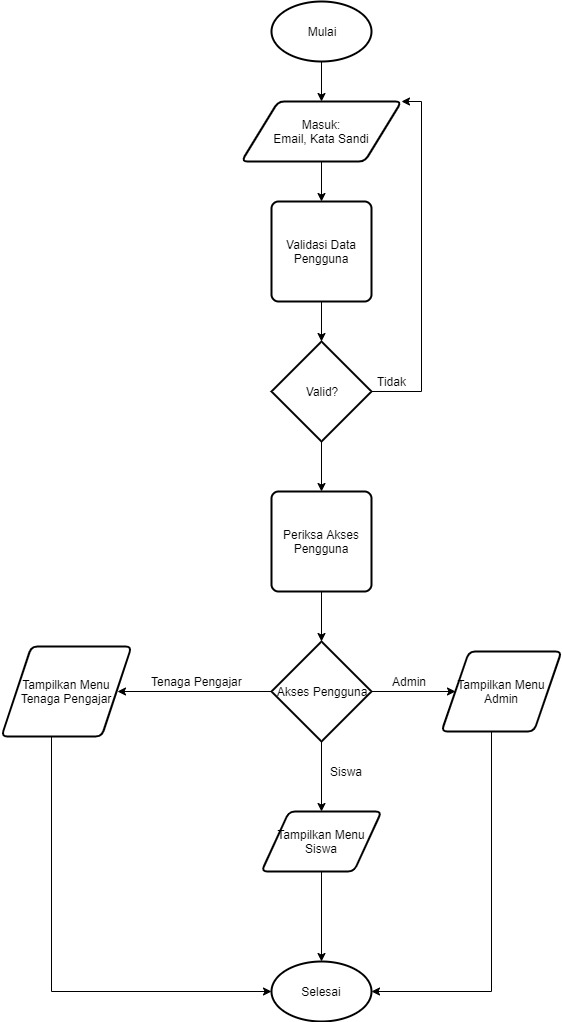
\includegraphics[width=15cm, height=18cm]{FlowChart.jpg}
		
		
		\subsubsection{Tabel}
			\centering
				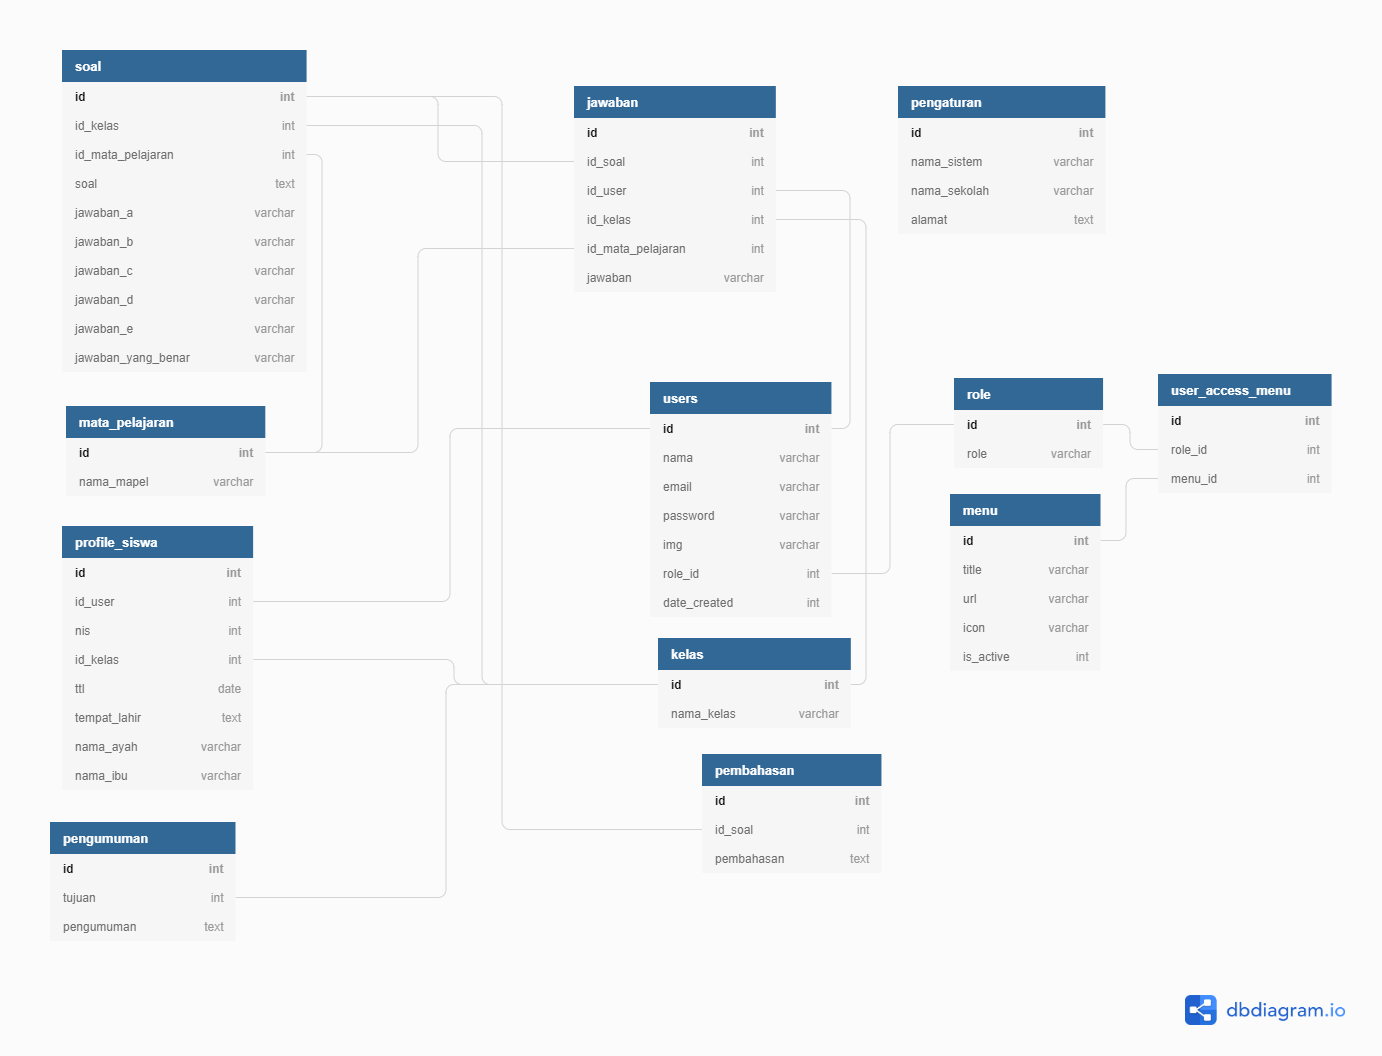
\includegraphics[width=17cm, height=15cm]{database-wbt.png}
		
		
		\subsubsection{UML}
		
		\begin{figure}
			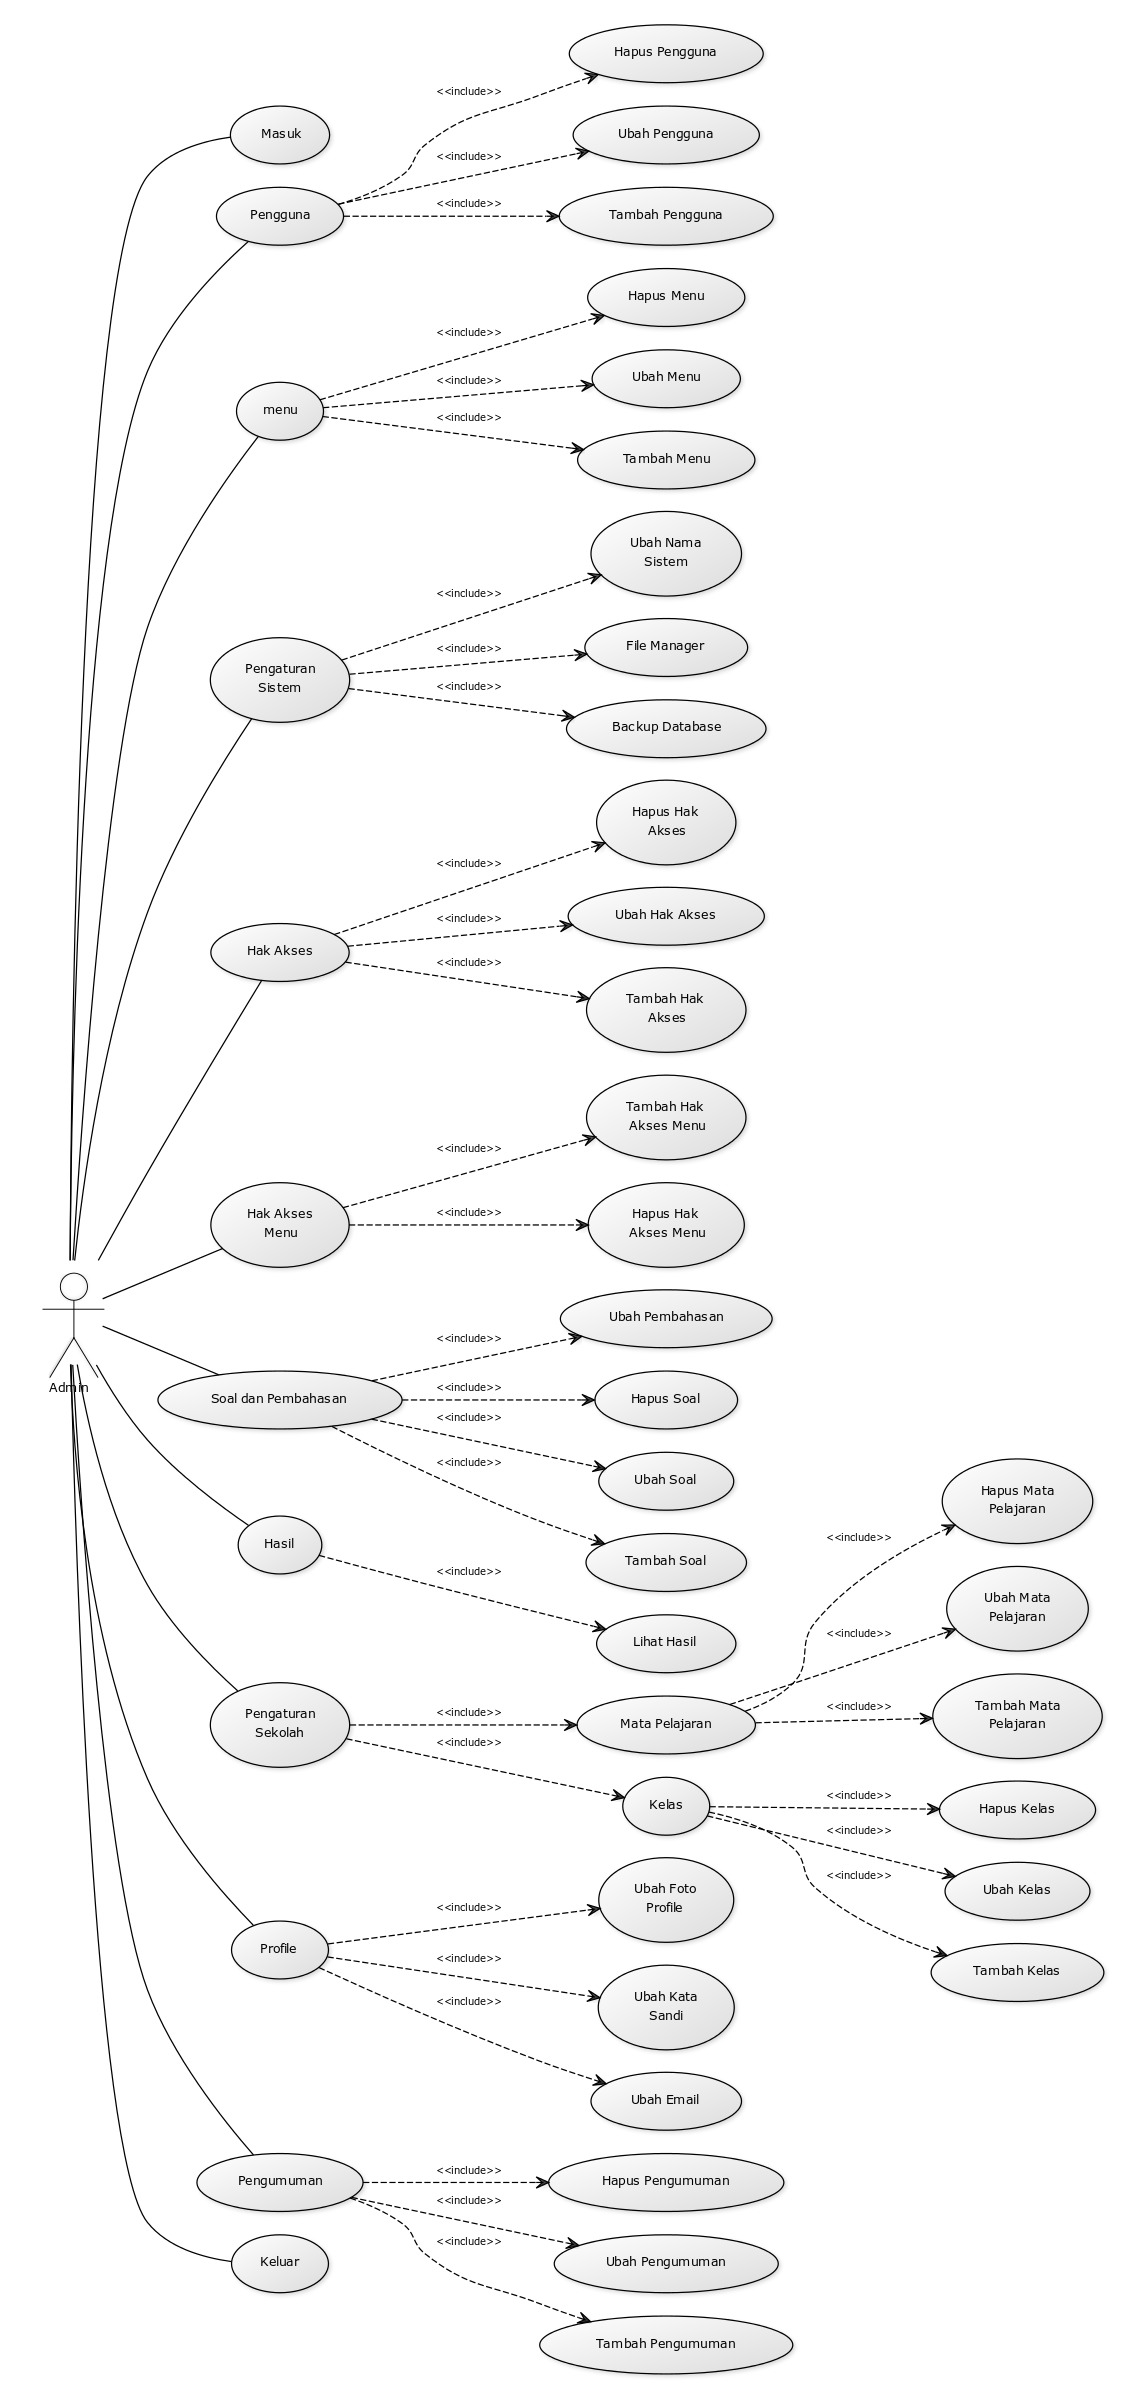
\includegraphics[width=18cm, height=20cm]{usecase-admin.jpg}
			\caption{Use Case Bagian Admin.}
		\end{figure}
	
		\begin{figure}
			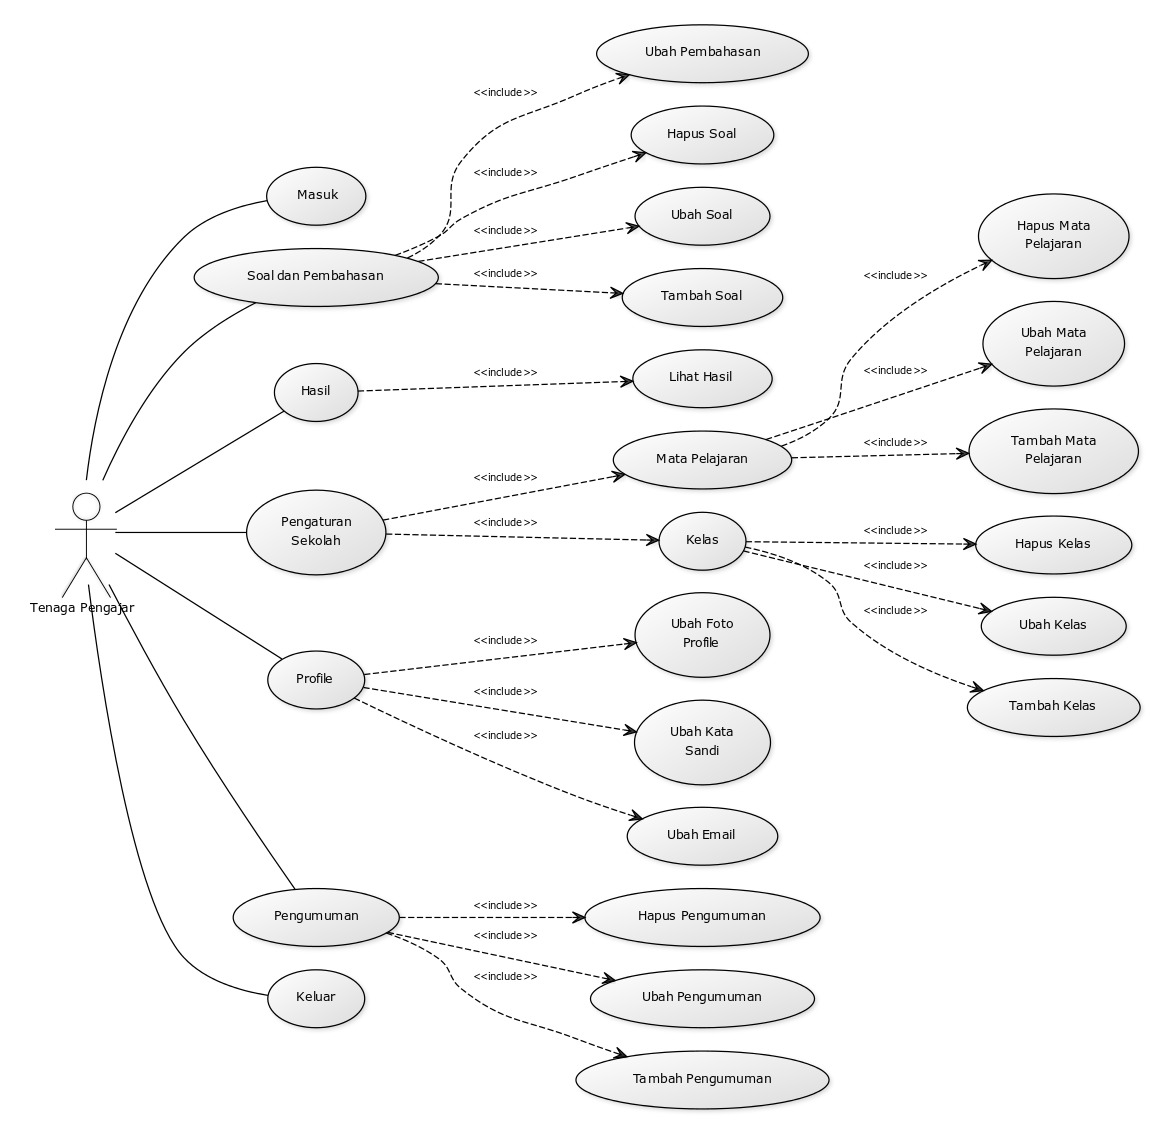
\includegraphics[width=18cm, height=20cm]{usecase-tenaga-pengajar.jpg}
			\caption{Use Case Bagian Tenaga Pengajar}
		\end{figure}
	
		\begin{figure}
			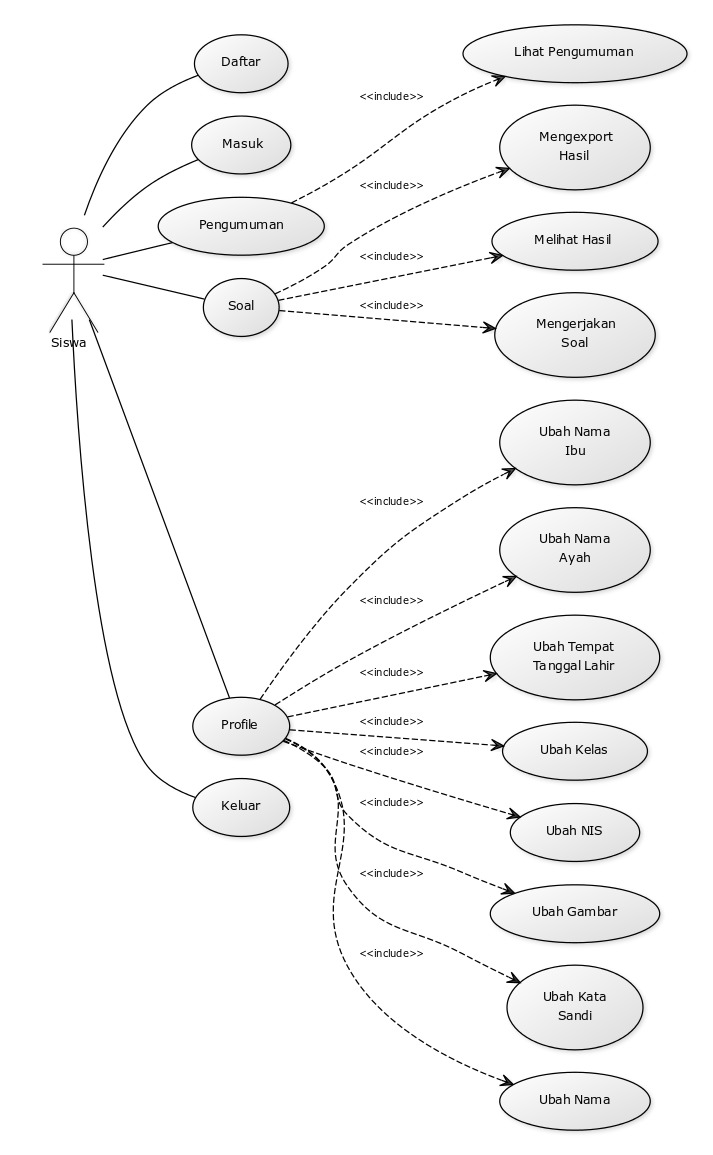
\includegraphics[width=18cm, height=20cm]{usecase-siswa.jpg}
			\caption{Use Case Bagian Siswa}
		\end{figure}
	
	
		\begin{figure}
			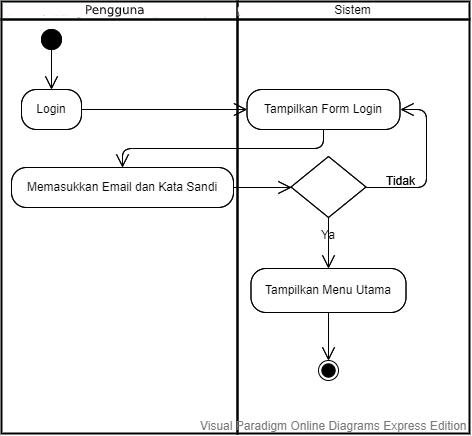
\includegraphics[width=15cm, height=20cm]{Activity-diagram-login.png}
			\caption{Activity Diagram \emph{Login}}
		\end{figure}
	
		\begin{figure}
			\includegraphics[width=15cm, height=20cm]{Activity-diagram-penambahan-soal.png}
			\caption{Activity Diagram Penambahan Soal}
		\end{figure}
	
		\begin{figure}
			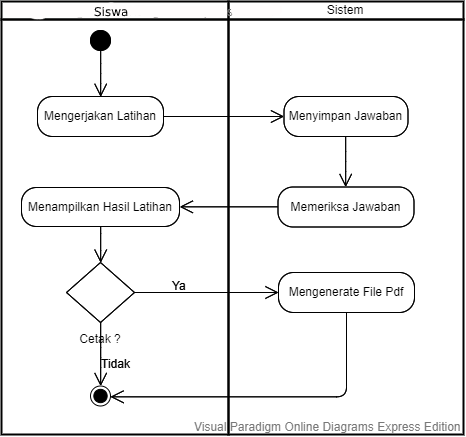
\includegraphics[width=15cm, height=20cm]{Activity-diagram-latihan.png}
			\caption{Activity Diagram Pengerjaan Soal}
		\end{figure}
		
		\begin{enumerate}
			\item Use Case
			\item Activity Diagram
			\item Class Diagram
			\item Sequence Diagram
		\end{enumerate}
	
	\subsection{Rancangan User Interface}

	


\end{document}
